% ========================================
\begin{figure*}[t!]
  \centering
  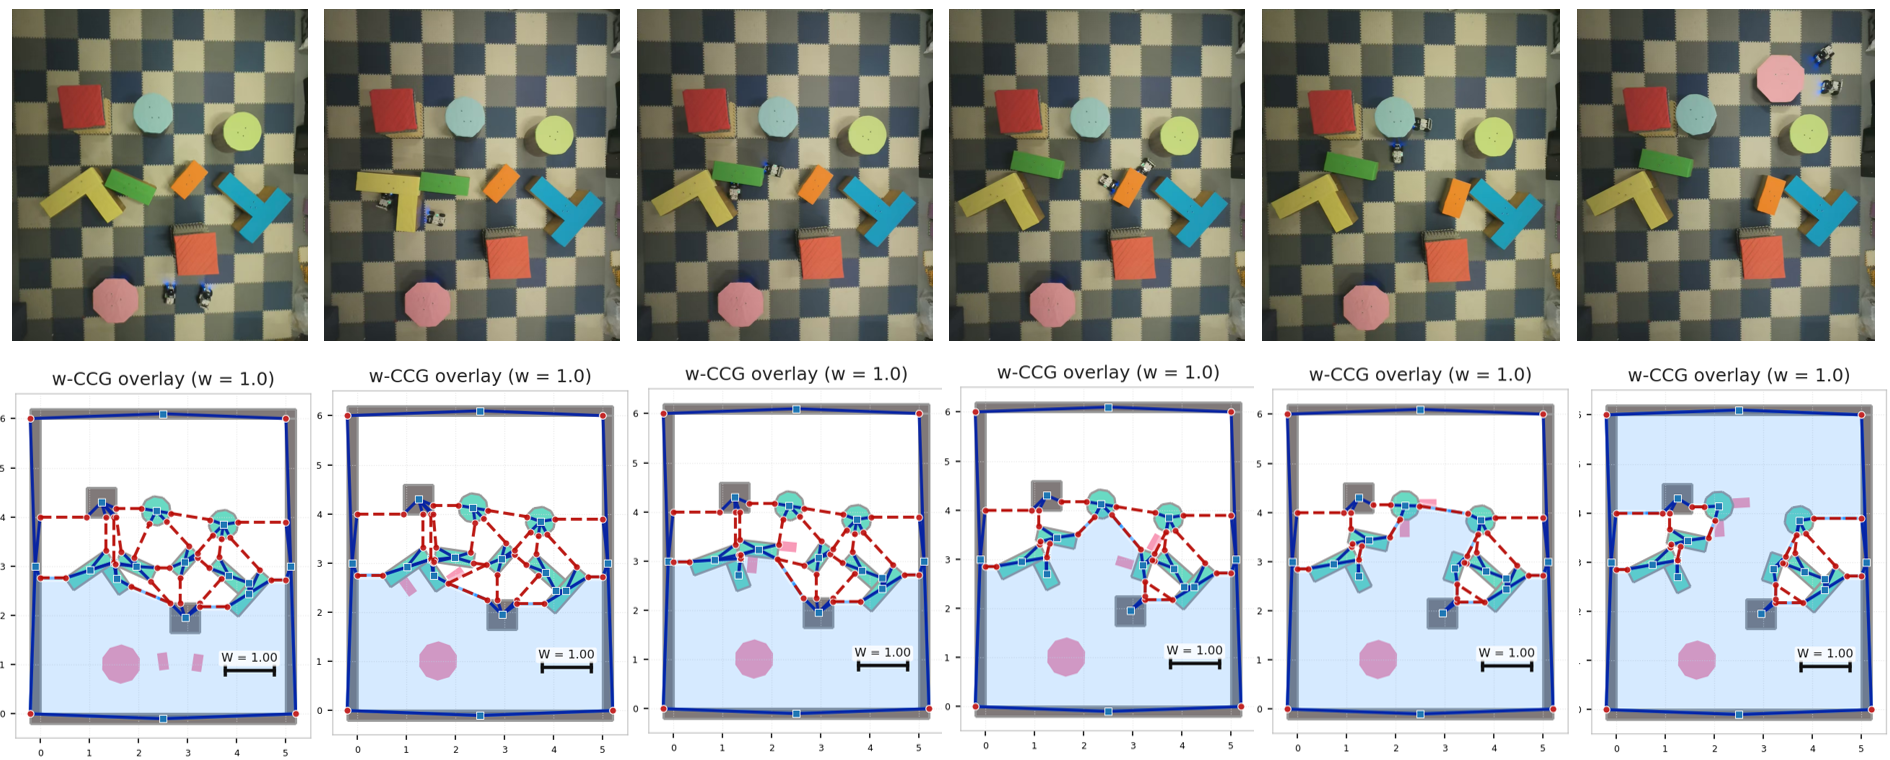
\includegraphics[width=0.95\linewidth]{figures/hardware_wccg.png}
  \vspace{-4mm}
  \caption{Real-world pushing experiment with execution--planning alignment.
\textbf{Top:} snapshots of two robots pushing obstacles in a \(5{\times}6\,\mathrm{m}\) workspace
with movable objects and fixed boundaries. \textbf{Bottom:} WCCG overlays with the start face in
blue. Planning uses clearance \(W{=}1.0\), start \(\mathbf{s}^{\texttt{S}}_{\texttt{V}}{=}(1.65,1.01)\),
and goal \(\mathbf{s}^{\texttt{G}}_{\texttt{V}}{=}(3.4,4.8)\).
The evolving graph remains consistent with observed motions, confirming that planned corridors
match execution.}
  \vspace{-4mm}
  \label{fig:hardware}
\end{figure*}
% ========================================
% ============================================================
\section{Experiments}
\label{sec:experiments}
We evaluate the proposed physics-informed hybrid search(PIHS)
in cluttered environments containing both movable
and immovable obstacles. All components—W-CCG presearch, frontier extraction,
and the \textit{ModeTable} prior—are integrated as described in Sec.~\ref{sec:solution}.
The implementation is in \texttt{Python~3};
simulations run in \texttt{PyBullet}~\cite{coumans2019} on a laptop with an Intel Core i7\textendash1280P CPU.
Videos and logs are provided in the supplementary material.



\subsection{Numerical Simulation}
\label{subsec:sim}
% ========================================

\subsubsection{Setup and Configuration}\label{subsec:sim-setup}
As shown in Fig.~\ref{fig:simloop},
the simulation has a step of $\Delta t=1/240$\,s and a control period of $1/40$\,s. Robots
are modeled as disk or box pushers with radii consistent with the $W$-clearance definition. Movable
obstacles have masses uniformly sampled from $[5,15]$\,kg, while immovables are modeled with zero
mass. A trial is successful when a $W$-clear path exists from start to goal and the target reaches
its goal disc. The nominal scenario consists of an $8{\times}5$\,m bounded workspace with two bar
obstacles forming bottlenecks and a mixed pool of curved and polygonal shapes including rings,
ellipses, X/T/L/diamond, arrow-like, rectangles, and cylinders. Two robots start in the lower-left
and the goal lies on the right, with $10$--$15$ movables placed randomly under a minimum separation.
The per-task simulation horizon is $80$ steps, and up to $64$ candidate push tasks are generated per
expansion. The node priority follows~\eqref{eq:priority} with heuristic factor
$10$, and gap sampling follows a softmax distribution with temperature~$0.05$. ModeTable is enabled
and automatically updated when missing. A quick-pass geometric screen skips physics if a reference
rollout already clears a gap; otherwise a short-horizon simulation with early stop is applied. To
prevent premature termination, a reinsertion rule preserves high-value nodes that cannot be
expanded immediately and revisits them later.

% ========================================
\begin{table}[t]
  \centering
  \begin{threeparttable}
  \caption{Performance comparison and ablations.}
  \label{tab:main_ablation}
  \vspace{2pt}
  \setlength{\tabcolsep}{2.5pt}
  \renewcommand{\arraystretch}{0.95}
  \begin{tabular}{lccccc}
  \toprule
  Method / Variant & Succ.(\%) & PT (s) & ET(s) & \#Sims & \#Pushes \\
  \midrule
   DFS-WCCG             & 25.0  & $>$100.0  & 51.2     & $>$500    & 8.0   \\
  SL-Push (off-line)   & 62.5  & 0.06  & 44.1   & 0.0   & 7.0  \\
  SL-Push (sim)        & 75.0  & 18.2  & 64.6   & 20.0 & 10.0  \\
  Rec-NAMO             & 37.5  & 13.3  & 42.4   & 0.0   & 7.0  \\
  \textbf{PushAround (ours)} & \textbf{92.5} & \textbf{10.3} & \textbf{28.6} & \textbf{121.5} & \textbf{6.0} \\
  \midrule
  w/o presearch        & 85.0 & 16.9 & 35.2 & 178 & 7.0 \\
  w/o ModeTable        & 80.0 & 15.1 & 33.4  & 164 & 6.0 \\
  w/o quick-pass       & 90.0 & 23.6 & 41.9  & 208 & 6.0 \\
  w/o reinsertion      & 82.5 & 12.8 & 31.1  & 151 & 7.0 \\
  \bottomrule
  \end{tabular}
  \end{threeparttable}
  \vspace{-4mm}
\end{table}
% ========================================


\subsubsection{Comparisons and Ablation Studies}\label{subsec:comparisons}
In total $8$ planners are evaluated under the same $W$-clearance criterion and contact models. External
baselines are: \textbf{DFS-WCCG}, a simulation-in-the-loop depth-first search guided by the W-CCG
with four fixed axis-aligned pushes per movable, which scales poorly due to exponential branching;
\textbf{SL-Push (offline)}, which clears blockers by minimal displacements along a straight or
waypointed route without physics, planning quickly but yielding unrealizable executions;
\textbf{SL-Push (sim)}, which validates the same route with physics, improving feasibility but
requiring many simulations and long action sequences; and \textbf{Rec-NAMO}, which combines Dijkstra
routing with local push decomposition and edge pruning, producing faster plans than simulation-heavy
methods but often failing to establish a connected $W$-clear corridor in dense clutter. Internal
ablations remove key modules of \textbf{PushAround}: \textbf{w/o presearch}, which disables frontier extraction and
gap ranking; \textbf{w/o ModeTable}, which discards structured contact-mode priors; \textbf{w/o
quick-pass}, which forces full-horizon rollouts; and \textbf{w/o reinsertion}, which prevents
revisiting promising but previously failed nodes.

Table~\ref{tab:main_ablation} shows that our method achieves the highest success rate of $92.5\%$
with the lowest combined planning and execution time. DFS-WCCG reaches only $25\%$ success due to
exponential branching.
As detailed in Fig.~\ref{fig:baseline},
SL-Push offline is extremely fast but produces physically invalid solutions,
while SL-Push sim improves feasibility at heavy computational cost. Rec-NAMO is faster but often
fails to produce complete solutions. The ablations reveal that presearch and ModeTable are critical,
with success drops of $7.5\%$ and $12.5\%$ accompanied by increased simulations. Quick-pass reduces
runtime overhead by $86$ additional simulations and $13.3$\,s in planning with little effect on
success, while reinsertion sustains robustness by recovering from local dead ends, as success drops
by $10.0\%$ when removed. Overall, the comparisons confirm that frontier-based ranking, structured
contact priors, and selective simulation are essential for scalability and feasibility, and that
deferred reinsertion further strengthens reliability.


% ========================================
\begin{figure}[t!]
  \centering
  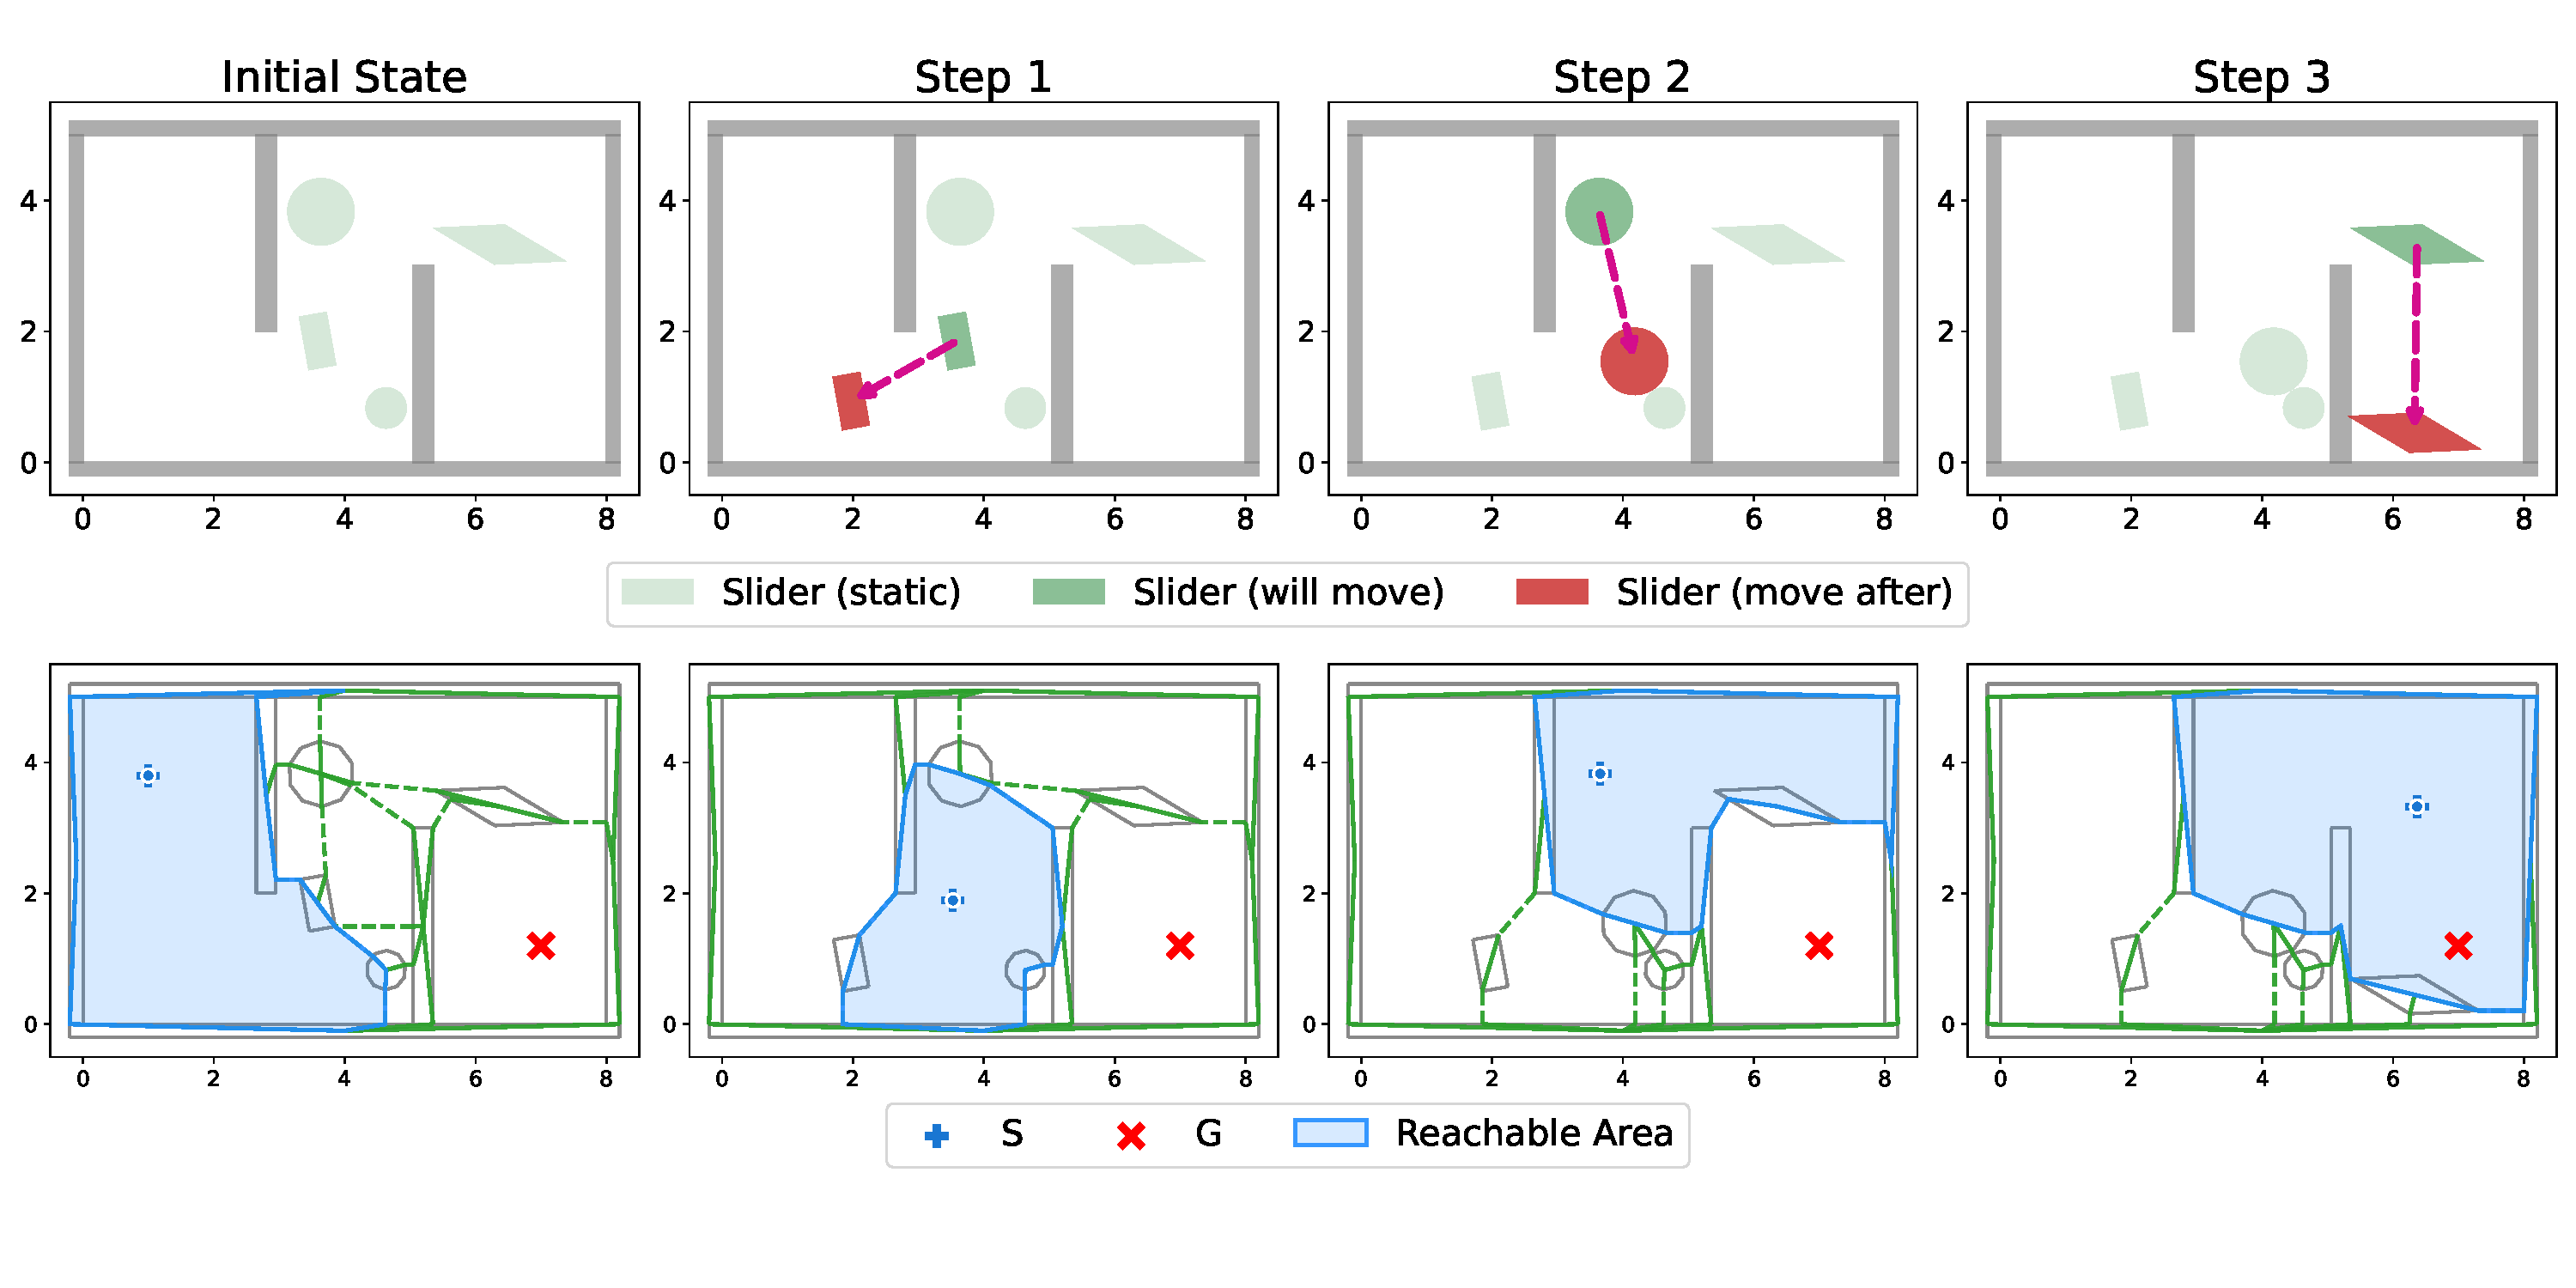
\includegraphics[width=0.95\columnwidth]{figures/Rec_NAMO.pdf}
  \vspace{-0.15in}
  \caption{\textbf{Left:} SL-Push, which determines pushing directions for movable obstacles along a $W$-width straight corridor between sub-start and sub-goal. \textbf{Right:} Rec-NAMO, which incrementally constructs path segments but often fails to establish a complete $W$-clear path from start to goal.}
  \vspace{-0.2in}
  \label{fig:baseline}
\end{figure}
% ========================================


\subsubsection{Scalability Analyses}\label{subsec:scalability}
Scalability is examined in an $8{\times}5$\,m workspace containing $30$ movable objects. Although
the combinatorial complexity increases, the WCCG presearch and the ModeTable guidance maintain a
small branching factor. As shown in Fig.~\ref{fig:scalability}, the run completes with $10$ node
expansions out of $115$ visited nodes, $312$ short simulation calls, and $7$ executed push tasks,
which yields a connected $W$-clear corridor. The planning time is $21.2$\,s and execution
$24.5$\,s, after which all robots reach the goal. These results confirm that the method sustains
efficiency and solution quality as scene density increases significantly.
% ========================================
\begin{figure}[t!]
  \centering
  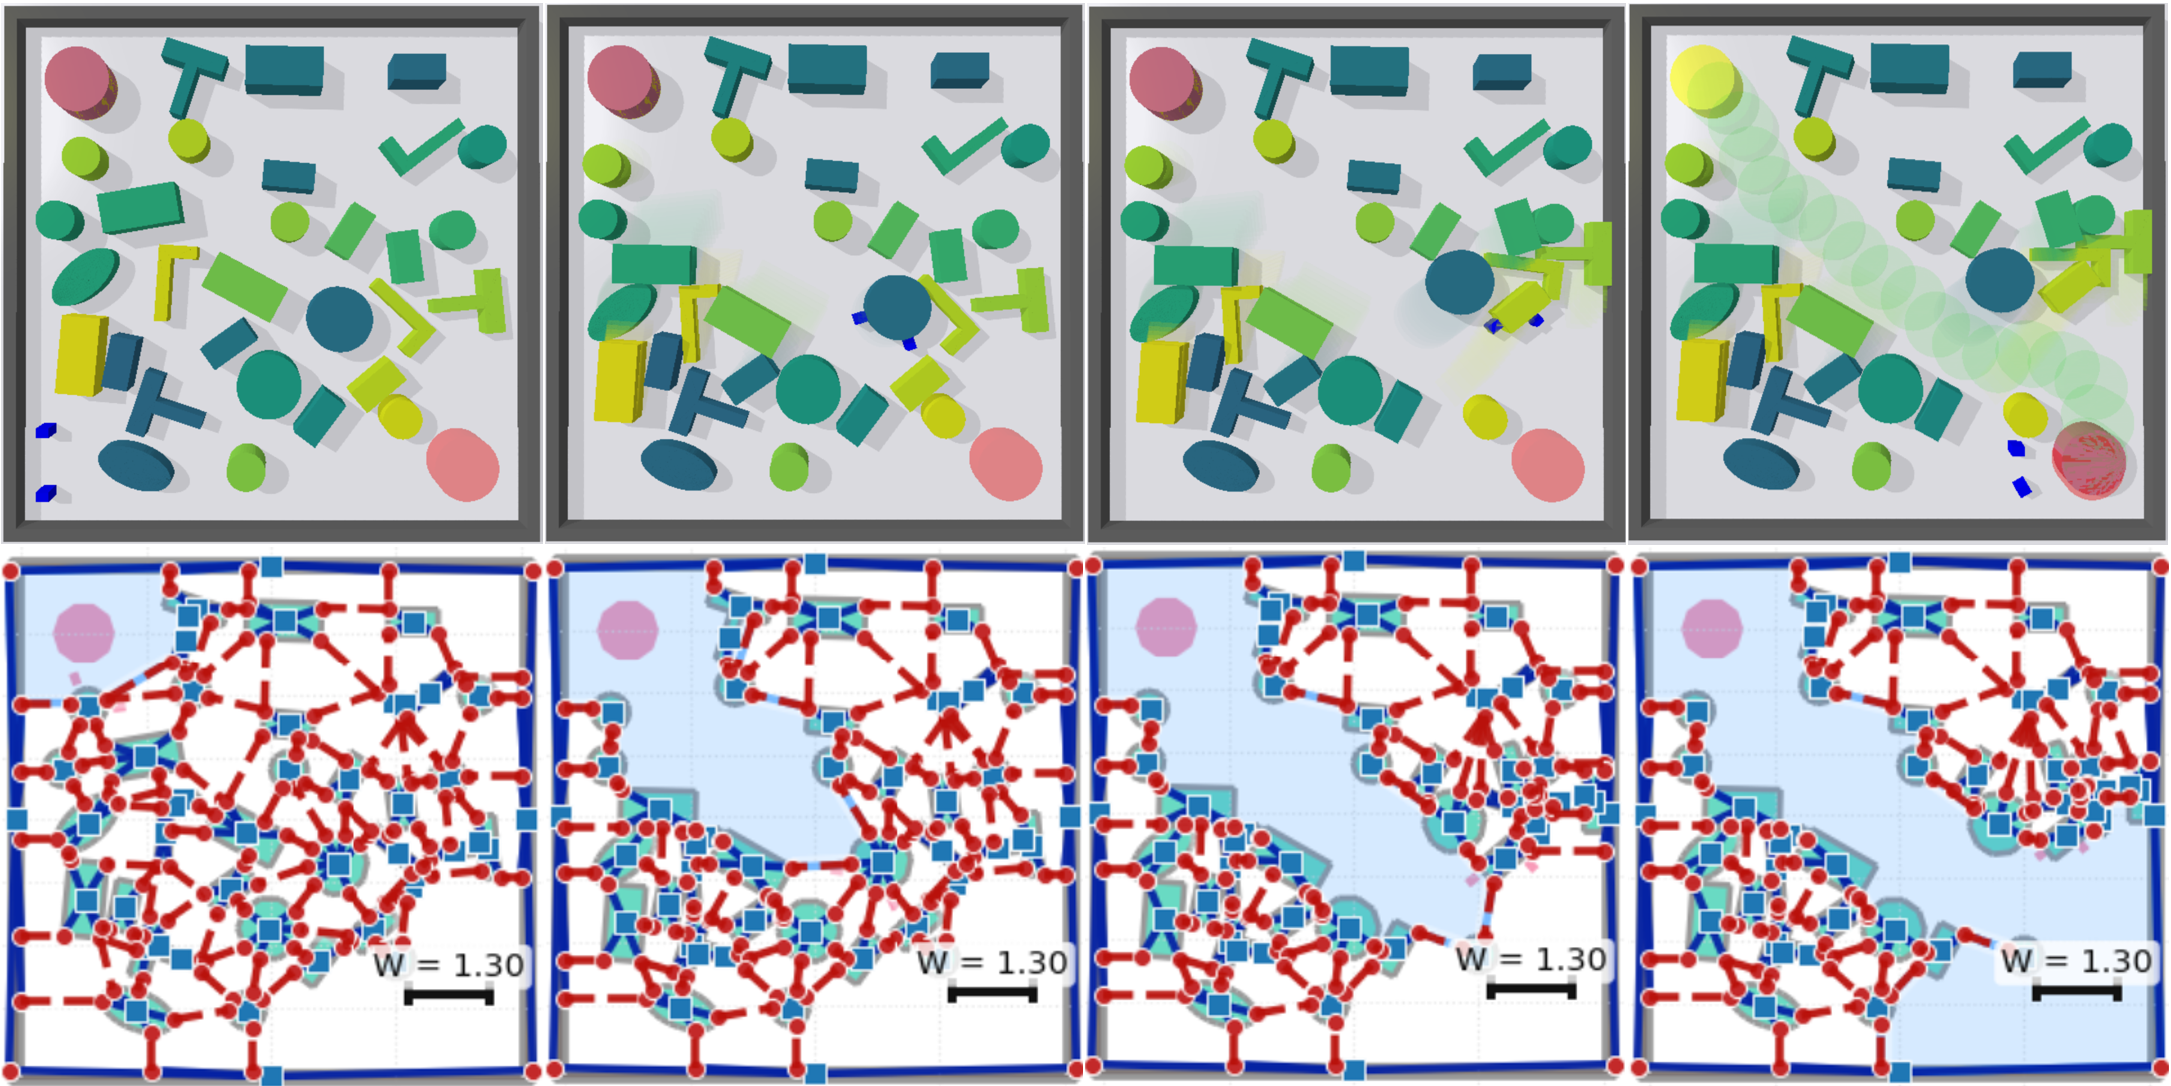
\includegraphics[width=0.95\linewidth]{figures/scalability.png}
  \vspace{-0.1in}
 \caption{Scalability in dense clutter with $\boldsymbol{30}$ movable objects.
\textbf{Top:} snapshots during the path clearing of $24.5$~s.
\textbf{Bottom:} WCCG overlays with the active face in blue and ranked frontier gaps.}
\label{fig:scalability}
\vspace{-0.2in}
\end{figure}
% ========================================


% ========================================
\subsection{Hardware Experiments}\label{subsec:hardware}
% ========================================

\subsubsection{System description}\label{subsec:exp-description}
Experiments are conducted in a $5\,\mathrm{m}\times6\,\mathrm{m}$ workspace assembled from
interlocking $0.6\,\mathrm{m}\times0.6\,\mathrm{m}$ foam mats, as illustrated in
Fig.~\ref{fig:hardware}. Each trial employs $2$ UGVs and $6$ movable obstacles
represented by cardboard boxes covered with colored paper for visual distinction. Both robots and
movables are equipped with three to four motion-capture markers. A motion-capture system streams
global poses to \texttt{PyBullet} in real time, enabling policy execution and visualization.
Movables are randomly placed at the beginning of each trial to generate diverse clutter.

\subsubsection{Results}\label{subsec:exp-results}
A representative real-world run is shown in Fig.~\ref{fig:snapshots} and~\ref{fig:hardware}.
The WCCG presearch completes
within $10$\,s, during which \textbf{$5$ gaps} are sequentially cleared through $64$ node expansions and a
maximum search depth of three. In the first task at $20$\,s, a yellow T-shaped object is rotated
counter-clockwise to expose a reachable contact on an adjacent green rectangle. In the second task
at $55$\,s, the green rectangle is pushed to its target. The third and fourth tasks manipulate an
orange rectangle and a blue cylinder at $71$\,s and $77$\,s, respectively, to open the
gaps. By the $5$-th task, all gaps in the WCCG are cleared, enabling a collision-free traverse from
start to goal. Execution time varies due to occasional drifting or slippage of the Mecanum wheels
near $45^\circ$, which lengthens certain transitions and introduces small deviations from simulation.
Online replanning compensates for these effects. The sequence of pushing actions and contact modes
confirms that the planned interactions are physically realizable on hardware.



% \begin{figure}[t]
%   \centering
%   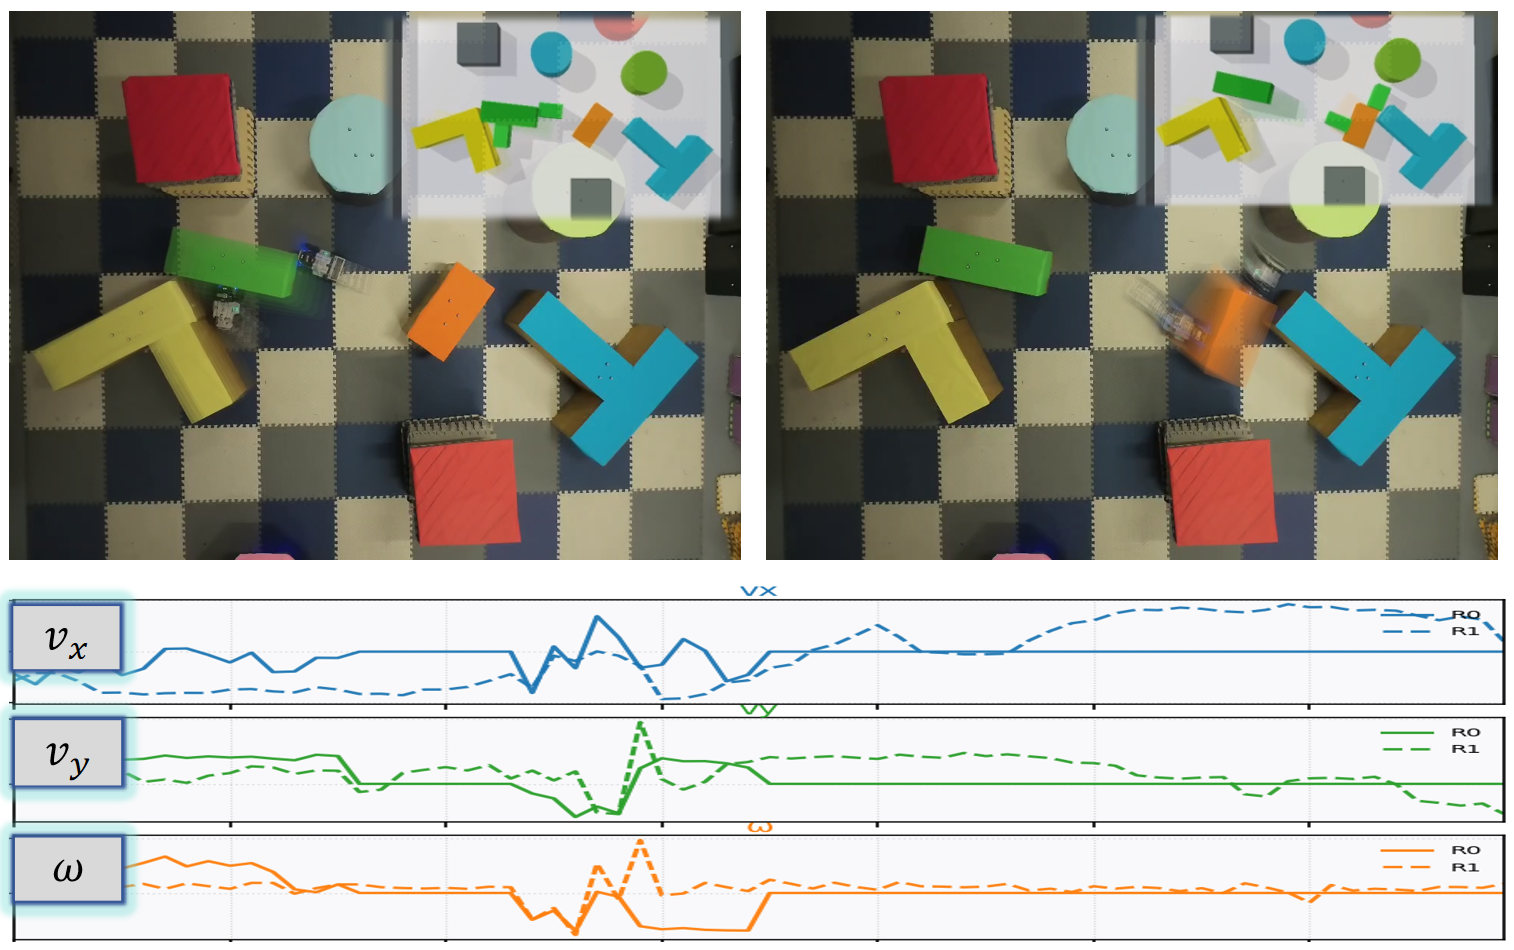
\includegraphics[width=\linewidth]{figures/hardware_snap.png}
%   \vspace{-2mm}
%   \caption{\textbf{Top:} two consecutive snapshots illustrating a chain push: R1 pushes an object, which then moves a neighbor. \textbf{Bottom:} velocity commands for both robots (\(v_x,v_y,\omega\)); the contact moment aligns with a brief rise in translational speed and differential angular commands.}
%   \label{fig:hardware_snap}
% \end{figure}
